\documentclass[12pt,a4paper]{article}
\usepackage[T2A]{fontenc}
\usepackage[utf8]{inputenc}
\usepackage[russian]{babel}
\usepackage[left=25mm,right=15mm,top=20mm,bottom=20mm]{geometry}
\usepackage{amsmath,amssymb,amsthm,mathtools}
\usepackage{graphicx}
\usepackage{float}
\usepackage{enumitem}
\usepackage{booktabs}
\usepackage{caption}
\usepackage[hidelinks]{hyperref}

\graphicspath{{fig/}}
\captionsetup{labelsep=period}
\setlength{\parindent}{1.25cm}
\linespread{1.15}

%\providecommand{\tg}{\mathop{\mathrm{tg}}\nolimits}
%\providecommand{\arctg}{\mathop{\mathrm{arctg}}\nolimits}
\newcommand{\sat}{\mathop{\mathrm{sat}}\nolimits}
\newtheorem*{remark}{Замечание}

\begin{document}
	
	% ================= ТИТУЛЬНЫЙ ЛИСТ =================
	\begin{titlepage}
		\begin{center}
			\small Министерство образования и науки Российской Федерации\\[2mm]
			\normalsize
			ФЕДЕРАЛЬНОЕ ГОСУДАРСТВЕННОЕ АВТОНОМНОЕ ОБРАЗОВАТЕЛЬНОЕ\\
			УЧРЕЖДЕНИЕ ВЫСШЕГО ОБРАЗОВАНИЯ\\[3mm]
			САНКТ-ПЕТЕРБУРГСКИЙ НАЦИОНАЛЬНЫЙ\\
			ИССЛЕДОВАТЕЛЬСКИЙ УНИВЕРСИТЕТ ИНФОРМАЦИОННЫХ\\
			ТЕХНОЛОГИЙ,\\
			МЕХАНИКИ И ОПТИКИ
			
			\vspace{20mm}
			{\Large\bfseries ЗАДАНИЕ № 2}
			
			\vspace{4mm}
			{\small по курсу: <<Нелинейные системы управления>>}
			
			\vspace{8mm}
			{\large\bfseries УСТОЙЧИВОСТЬ НЕЛИНЕЙНЫХ СИСТЕМ:\\
				ФУНКЦИИ ЛЯПУНОВА, LMI\\
				И УСТОЙЧИВОСТЬ ПО ВХОДУ К СОСТОЯНИЮ}
			
			\vspace{30mm}
			\hfill
			\begin{tabular}{ll}
				Авторы работы: & Титаренко П. А.\\
				& Охрименко Е. Д.\\[2mm]
				Преподаватель: & Зименко Константин Александрович
			\end{tabular}
		\end{center}
		
		
		\vfill
		\begin{center}
			Санкт-Петербург\\
			2026 г.
		\end{center}
	\end{titlepage}
	
	\tableofcontents
	\newpage
	
	% =================================================
	\section{Исследование устойчивости с помощью квадратичной функции Ляпунова}
	
	\textbf{Условие.} Для каждой из систем использовать кандидат квадратичной функции Ляпунова,
	чтобы показать, что начало координат асимптотически устойчиво. Определить, в каких случаях
	система глобально устойчива в начале координат.
	
Функция $V(x)=x_1^2+x_2^2$ положительно определена и радтально неограничена, а её производная отрицательно определена во всей области.
	
\subsection{Система 1}
\[
\begin{cases} 
	\dot x_1=-x_1+x_1x_2 \\ 
	\dot x_2=-2x_2 
\end{cases}
\]

Берём $V=x_1^2+x_2^2$. Производная в силу системы:
\[
\dot V = 2x_1(-x_1+x_1x_2)+2x_2(-2x_2) = -2x_1^2(1-x_2)-4x_2^2.
\]

При $x_2<1$ скобка $(1-x_2)>0$, поэтому $\dot V<0$ при всех $x\neq0$. Начало координат асимптотически устойчиво. Оценка области притяжения — наибольший круг внутри полосы $x_2<1$: $\Omega_1=\{x_1^2+x_2^2<1\}$.

Квадратичная функция не доказывает глобальность (при $x_2>1$ знак $\dot V$ не определён). 
Но система решается явно: из второго уравнения
\[
x_2(t)=x_2(0)e^{-2t}\to0,
\]
а первое уравнение линейно по $x_1$. Подставляя решение для $x_2$, получаем
\[
x_1(t)=x_1(0)\exp\!\left(-t+\frac{x_2(0)}{2}(1-e^{-2t})\right)\to0 \quad \text{при } t\to\infty.
\]
Следовательно, начало координат глобально асимптотически устойчиво.
	
\subsection{Система 2}
\[
\begin{cases} 
	\dot x_1=-x_2-x_1(1-x_1^2-x_2^2) \\ 
	\dot x_2=x_1-x_2(1-x_1^2-x_2^2)
\end{cases}
\]

Берём $V=x_1^2+x_2^2=r^2$. Производная в силу системы:
\[
\dot V = 2x_1\dot x_1+2x_2\dot x_2 = -2r^2(1-r^2).
\]

При $0<r<1$ имеем $\dot V<0$, значит, начало координат асимптотически устойчиво. Оценка области притяжения — открытый единичный круг $\Omega_1=\{x_1^2+x_2^2<1\}$.

При $r>1$ знак $\dot V$ положительный, траектории уходят на бесконечность. Окружность $r=1$ является неустойчивым предельным циклом ($\dot V=0$, $\dot\varphi=1$). Следовательно, глобальной устойчивости нет.
	
\subsection{Система 3}
\[
\begin{cases} 
	\dot x_1=x_2(1-x_1^2)-2x_1 \\ 
	\dot x_2=-(x_1+x_2)(1-x_1^2)
\end{cases}
\]

Берём $V=x_1^2+x_2^2$. Производная в силу системы:
\[
\dot V = 2x_1[x_2(1-x_1^2)-2x_1] + 2x_2[-(x_1+x_2)(1-x_1^2)] = -4x_1^2-2x_2^2(1-x_1^2).
\]

При $|x_1|<1$ имеем $(1-x_1^2)>0$, поэтому $\dot V<0$ при всех $x\neq0$. Начало координат асимптотически устойчиво. Оценка области притяжения — наибольший круг внутри полосы $|x_1|<1$: $\Omega_1=\{x_1^2+x_2^2<1\}$.

Глобальной устойчивости нет, так как существуют другие положения равновесия. Из условия $\dot x=0$ находим точки $(\sqrt3,-\sqrt3)$ и $(-\sqrt3,\sqrt3)$, которые не принадлежат $\Omega_1$.


\subsection{Система 4}
\[
\begin{cases} 
	\dot x_1=-3x_1-x_2 \\ 
	\dot x_2=2x_1-x_2^3 
\end{cases}
\]

Берём взвешенную функцию $V(x)=2x_1^2+x_2^2$. Производная в силу системы:
\[
\dot V = 4x_1(-3x_1-x_2)+2x_2(2x_1-x_2^3) = -12x_1^2-2x_2^4.
\]

Функция $V$ положительно определена и радиально неограничена, а $\dot V$ отрицательно определена во всём $\mathbb R^2$. Следовательно, начало координат глобально асимптотически устойчиво.
	
\subsection{Система 5}
\[
\dot x=-\arctg x .
\]

Для $V=x^2$ производная равна $\dot V=-2x\arctg x$. Так как $\arctg x$ имеет тот же знак, что и $x$, то $\dot V<0$ при всех $x\neq0$. Функция $V$ радиально неограничена, значит, система глобально асимптотически устойчива.
	
	\begin{figure}[H]
		\centering
		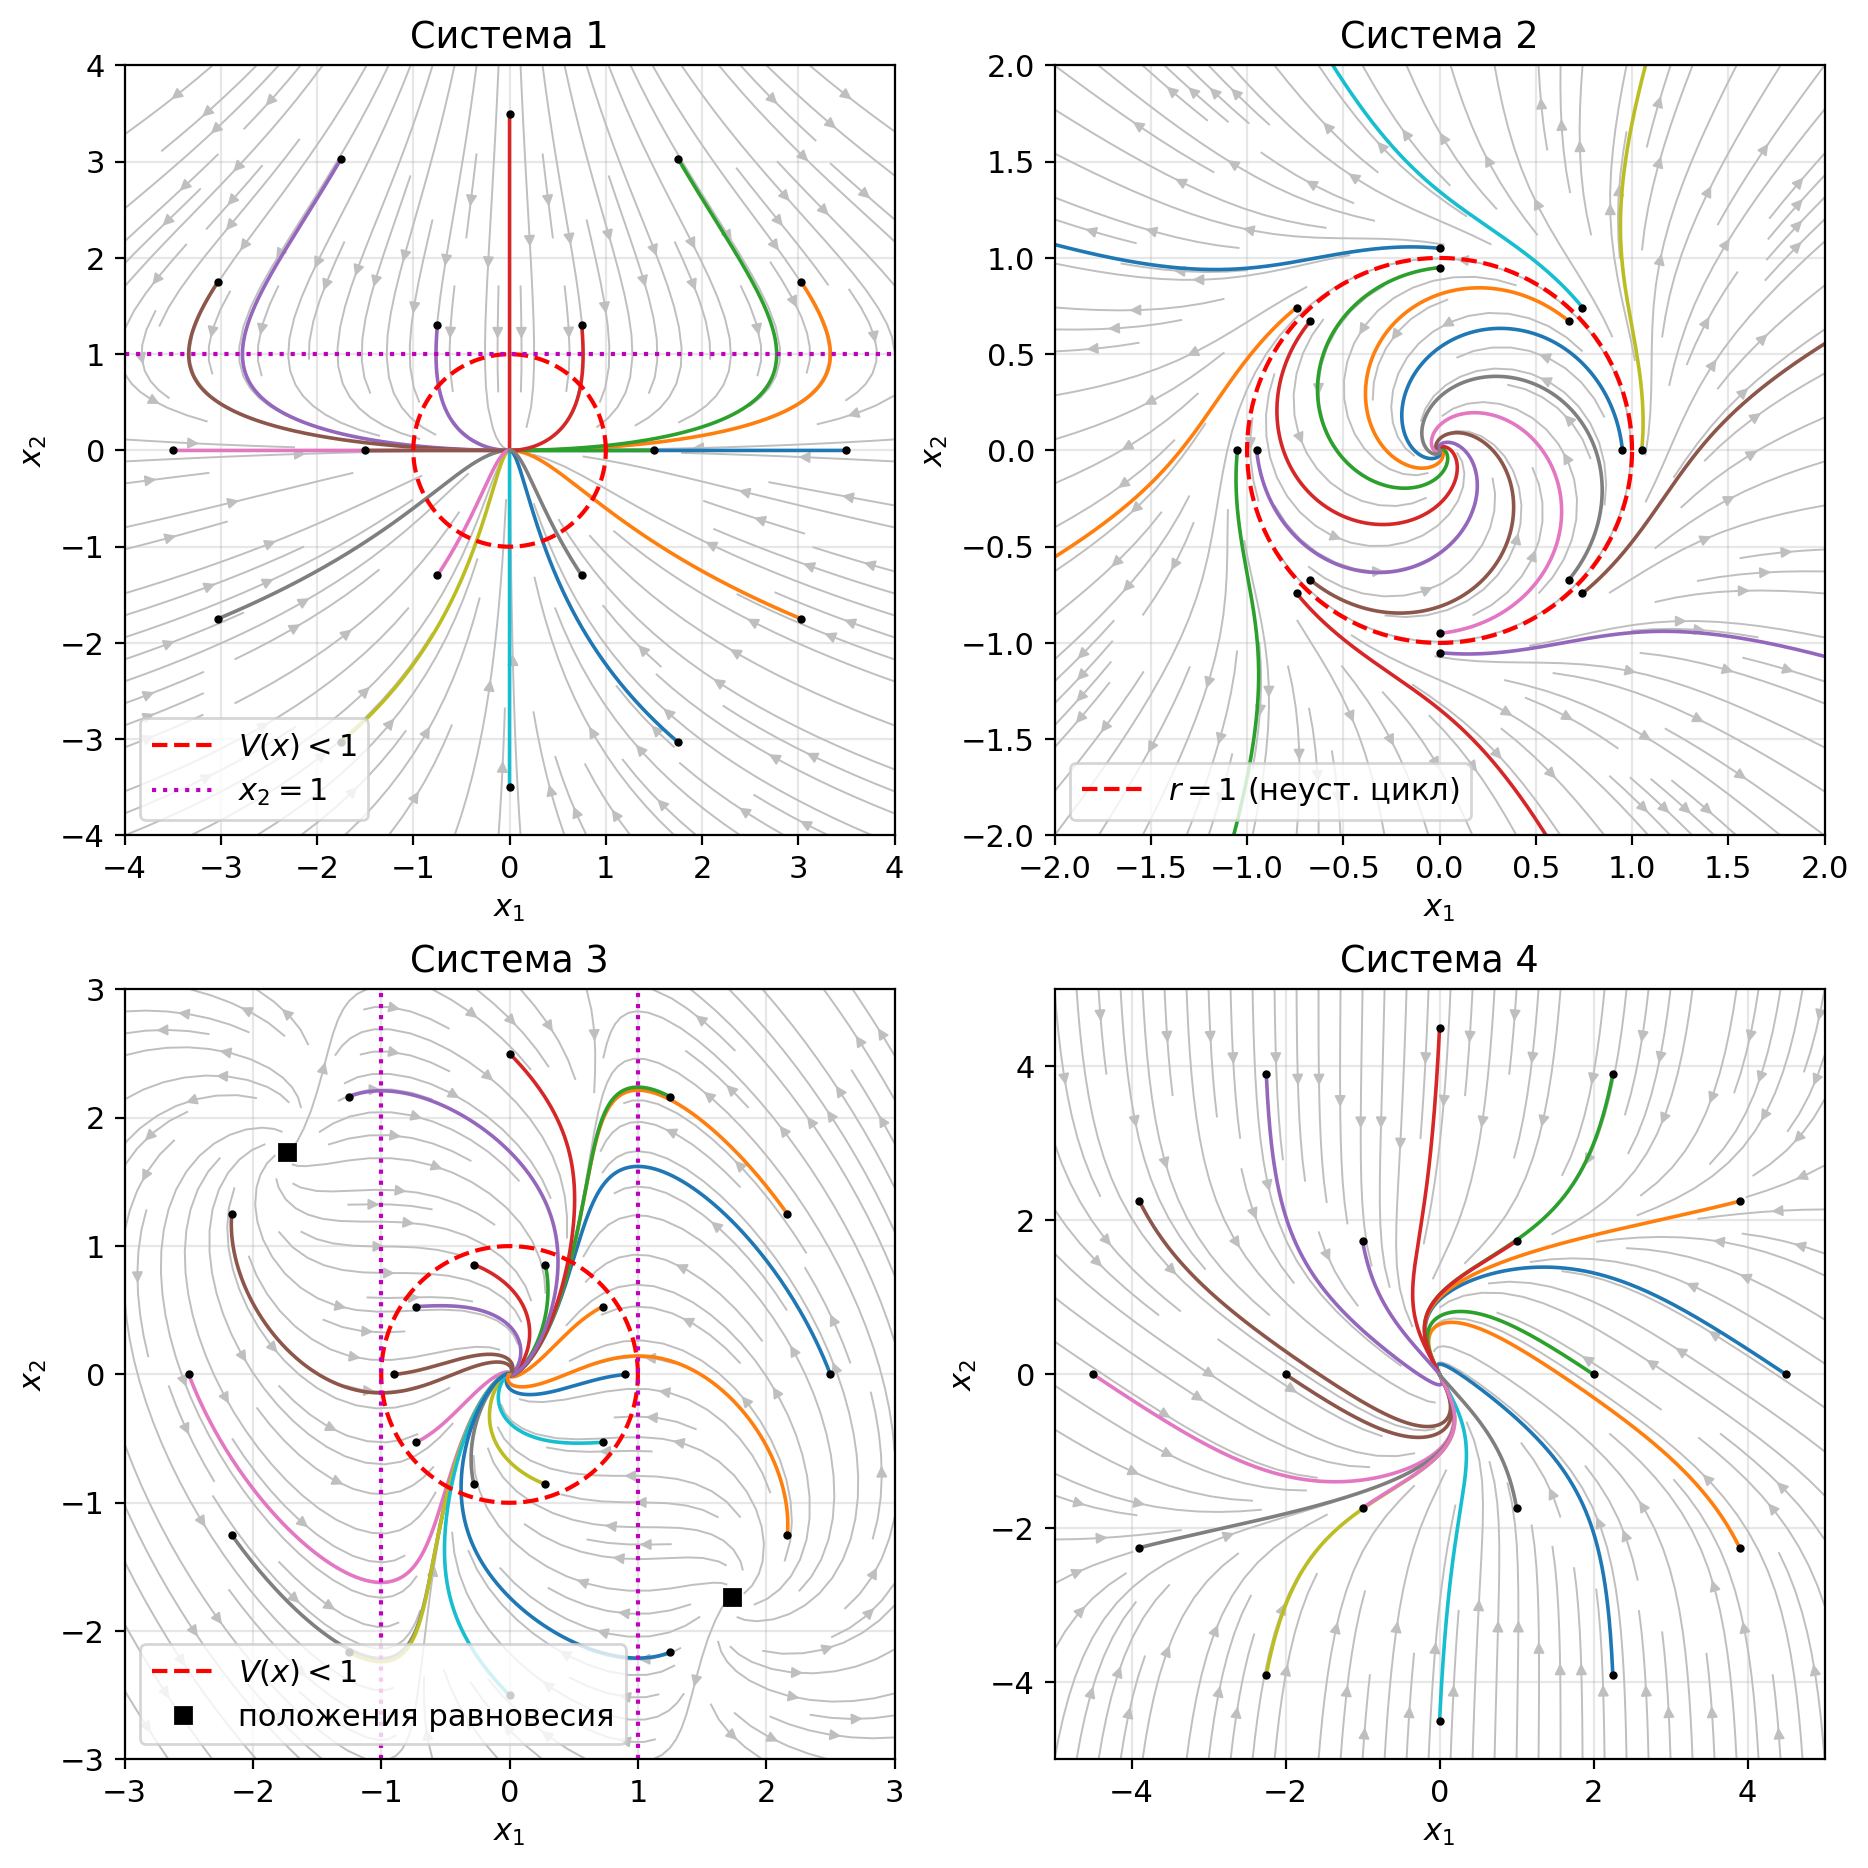
\includegraphics[width=0.95\textwidth]{../images/task1_portraits.png}
		\caption{Фазовые портреты систем 1--4. Красный пунктир~--- оценки области притяжения
			(для системы 2~--- неустойчивый предельный цикл), квадраты~--- дополнительные положения равновесия системы 3}
		\label{fig:t1}
	\end{figure}
	
	\begin{figure}[H]
		\centering
		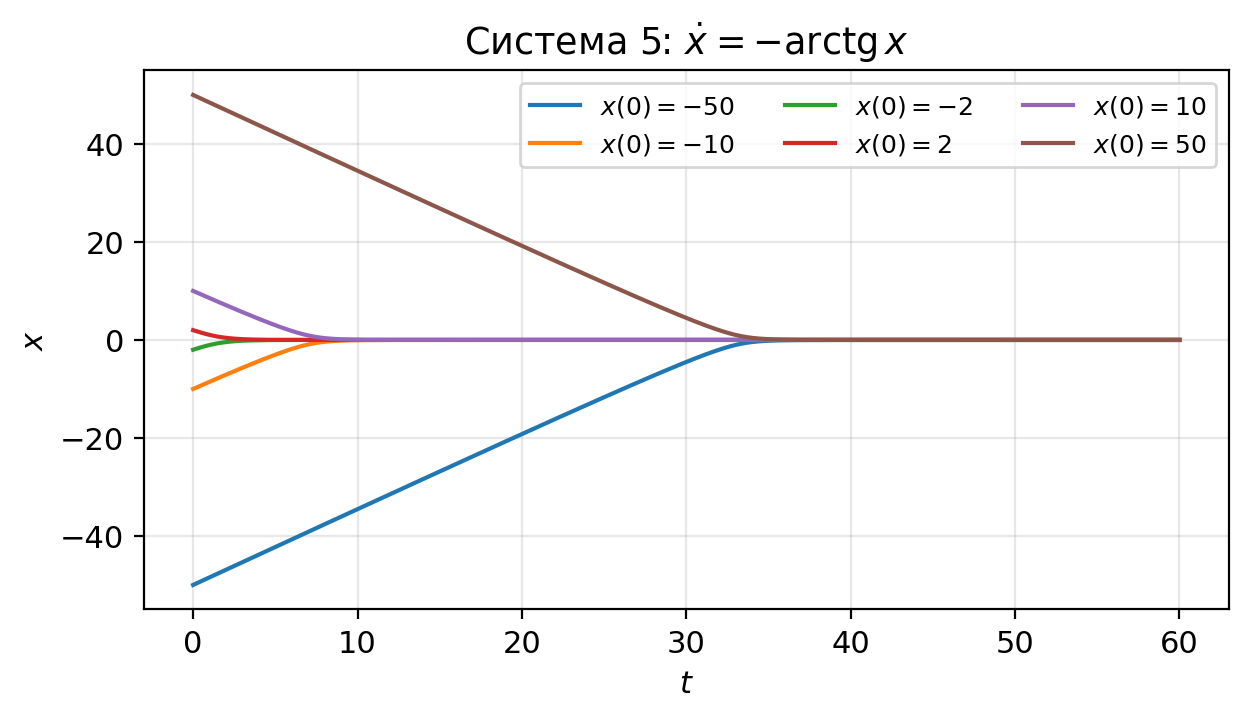
\includegraphics[width=0.7\textwidth]{../images/task1_sys5.png}
		\caption{Переходные процессы системы 5}
		\label{fig:t1s5}
	\end{figure}
	
\subsection{Вывод по заданию 1}
\begin{center}
	\begin{tabular}{cccl}
		\toprule
		Система & $V$ & Устойчивость & Обоснование \\
		\midrule
		1 & $x_1^2+x_2^2$ & глобальная АУ & явное решение системы \\
		2 & $x_1^2+x_2^2$ & локальная АУ & область притяжения $r<1$ \\
		3 & $x_1^2+x_2^2$ & локальная АУ & наличие других равновесий \\
		4 & $2x_1^2+x_2^2$ & глобальная АУ & $\dot V=-12x_1^2-2x_2^4$ \\
		5 & $x^2$ & глобальная АУ & $\dot V=-2x\arctg x$ \\
		\bottomrule
	\end{tabular}
\end{center}
Глобально асимптотически устойчивы системы 1, 4 и 5. Системы 2 и 3 устойчивы только локально из-за наличия неустойчивого предельного цикла и дополнительных положений равновесия соответственно.
	
	
	\newpage
\section{Скалярная система $\dot x = ax^p+h(x)$}


Рассмотрим функцию Ляпунова $V=\tfrac12x^2$. Её производная в силу системы:
\[
\dot V = ax^{p+1} + xh(x), \quad |xh(x)| \le k|x|^{p+2}.
\]

При нечётном $p$ и $a<0$ имеем $x^{p+1}=|x|^{p+1}$, откуда следует оценка:
\[
\dot V \le -|a||x|^{p+1} + k|x|^{p+2} = -|x|^{p+1}(|a|-k|x|).
\]
В области $0<|x|<|a|/k$ производная отрицательна, начало координат асимптотически устойчиво (экспоненциально при $p=1$, нет при $p\ge3$).

При нечётном $p$ и $a>0$:
\[
\dot V \ge |x|^{p+1}(a-k|x|) > 0.
\]
Так как $V(0)=0$ и $\dot V>0$, траектории удаляются от нуля, равновесие неустойчиво.

При чётном $p$ знак $ax^p$ одинаков по обе стороны от нуля, а $h(x)=o(x^p)$. На одной из полуосей $\dot V>0$, равновесие неустойчиво.

При $a=0$ главный член исчезает, устойчивость определяется видом $h(x)$.

Ответ: асимптотическая устойчивость достигается тогда и только тогда, когда $p$ нечётно и $a<0$.
	
	
	\newpage
\section{Синтез линейного регулятора на основе LMI}

Рассмотрим систему:
\[
\begin{cases} 
	\dot x_1=x_2 \\ 
	\dot x_2=2x_1+u 
\end{cases}
\]
в матричной форме $\dot x=Ax+Bu$, где
\[
A=\begin{pmatrix}0&1\\2&0\end{pmatrix}, \quad B=\begin{pmatrix}0\\1\end{pmatrix}.
\]
Пара $(A,B)$ управляема. Ищем статический регулятор $u=Kx$, обеспечивающий экспоненциальную устойчивость со степенью $\alpha=2$. Это условие эквивалентно выполнению неравенства Ляпунова для $V=x^\top Px$, $P\succ0$:
\[
(A+BK)^\top P + P(A+BK) + 2\alpha P \prec 0.
\]
Данное неравенство нелинейно по переменным $(P,K)$. Введём замену $Q=P^{-1}$, $Y=KQ$ и умножим неравенство слева и справа на $Q$. Получаем линейное матричное неравенство (LMI):
\[
\begin{cases} 
	Q \succ 0 \\ 
	AQ + QA^\top + BY + Y^\top B^\top + 2\alpha Q \prec 0 
\end{cases}
\]
Решая эту систему неравенств численно при $\alpha=2$, находим допустимые матрицы $Q$ и $Y$. Коэффициенты регулятора восстанавливаются как $K=YQ^{-1}$:
\[
K = \begin{pmatrix}-10.785 & -4.521\end{pmatrix}.
\]
Проверка подтверждает выполнение требований: собственные числа замкнутой матрицы $A+BK$ равны $-2.261 \pm 1.917i$ ($\operatorname{Re}\lambda < -2$), а неравенство Ляпунова выполняется строго. Следовательно, для траекторий замкнутой системы справедлива оценка:
\[
\|x(t)\| \le \sqrt{\frac{\lambda_{\max}(P)}{\lambda_{\min}(P)}} e^{-2t} \|x(0)\|.
\]

	
	\newpage
\section{Ограничение на параметр $\gamma$}

Рассмотрим замкнутую систему с регулятором из задания 3:
\[
\begin{cases} 
	\dot x_1 = x_2 + \gamma \sin x_2 \\ 
	\dot x_2 = 2x_1 + u, \quad u = Kx 
\end{cases}
\]
Требуется найти диапазон $\gamma$, при котором система экспоненциально устойчива со степенью $\beta=1$.

Представим нелинейность в виде $\sin x_2 = \theta(x_2) x_2$, где $\theta(x_2) = \dfrac{\sin x_2}{x_2}$ (при $x_2=0$ полагаем $\theta(0)=1$). Это позволяет записать систему как линейную с параметрической неопределенностью:
\[
\dot x = A(\theta)x, \quad A(\theta) = \begin{pmatrix} 0 & 1+\gamma\theta \\ 2+k_1 & k_2 \end{pmatrix}, \quad \theta \in [\theta_{\min}, 1],
\]
где $\theta_{\min} \approx -0.2172$.

Условие экспоненциальной устойчивости со степенью $\beta=1$ сводится к существованию общей матрицы Ляпунова $P \succ 0$, удовлетворяющей неравенству:
\[
A(\theta)^\top P + P A(\theta) + 2\beta P \prec 0.
\]
Так как это неравенство линейно по $\theta$, достаточно проверить его только на границах интервала $\{\theta_{\min}, 1\}$. Решая задачу допустимости LMI методом половинного деления по $\gamma$, получаем:
\[
-0.599 < \gamma < 1.364.
\]

Нижняя граница является точной: при $\gamma \le -0.599$ даже линеаризованная система ($\theta=1$) теряет требуемую степень устойчивости. Верхняя граница достаточна.
	
\newpage
\section{Синтез регулятора и устойчивость по входу к состоянию}

Рассматривается система
\[
\begin{cases} 
	\dot x_1 = x_2 - 0.5x_1^3 \\ 
	\dot x_2 = u, \quad u = Kx 
\end{cases}
\]
весь вектор состояния измеряется.

\subsection{Глобальная стабилизация}
Выбираем $K = (-1, -2)$. Замкнутая система имеет вид:
\[
\begin{cases} 
	\dot x_1 = x_2 - 0.5x_1^3 \\ 
	\dot x_2 = -x_1 - 2x_2 
\end{cases}
\]
Возьмём функцию Ляпунова $V(x) = x_1^2 + x_2^2$. Её производная в силу системы:
\[
\dot V = 2x_1(x_2 - 0.5x_1^3) + 2x_2(-x_1 - 2x_2) = -x_1^4 - 4x_2^2.
\]
Функция $V$ положительно определена и радиально неограниченна, а $\dot V$ отрицательно определена во всём $\mathbb{R}^2$. Следовательно, начало координат глобально асимптотически устойчиво.

\begin{figure}[H]
	\centering
	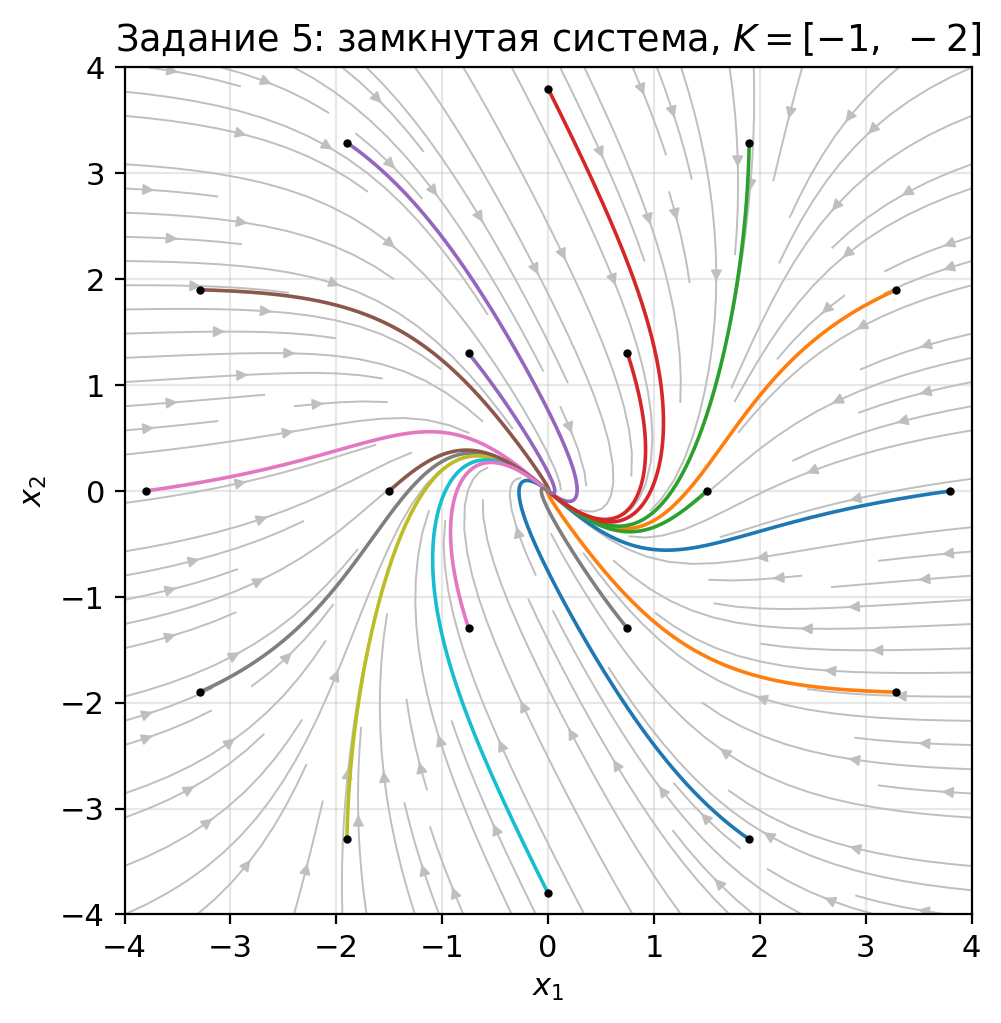
\includegraphics[width=0.55\textwidth]{../images/task5_portrait.png}
	\caption{Фазовый портрет замкнутой системы}
\end{figure}

\subsection{Шумы измерений}
Пусть измеряется $x+e$, где $e(t)$ --- ограниченный шум. Тогда $u=K(x+e)$ и
\[
\dot V = -x_1^4-4x_2^2 + 2x_2 K e \le -x_1^4-2x_2^2 + \tfrac{5}{2}|e|^2,
\]
где использовано неравенство $2ab \le 2a^2 + \tfrac{1}{2}b^2$ и $|K|^2=5$. 
Так как $x_1^4+2x_2^2$ положительно определена и радиально неограниченна, то при любом фиксированном уровне шума $\|e\|_\infty$ существует такая область $\Omega$, что вне её $\dot V < 0$. Следовательно, все траектории системы остаются ограниченными и входят в некоторую окрестность начала координат, размер которой зависит от уровня шума.


\subsection{Аддитивные возмущения}
Пусть \[\begin{cases}
	\dot x_1=x_2-0.5x_1^3+d_1 \\
	\dot x_2=Kx+d_2
\end{cases}\]

Тогда:
\[
\dot V = -x_1^4-4x_2^2 + 2x_1 d_1 + 2x_2 d_2.
\]
Используя: $2|x_1||d_1| \le \tfrac{1}{2}x_1^4 + 2d_1^2$ и $2x_2 d_2 \le 2x_2^2 + \tfrac{1}{2}d_2^2$, получаем:
\[
\dot V \le -\tfrac{1}{2}x_1^4 - 2x_2^2 + 2d_1^2 + \tfrac{1}{2}d_2^2.
\]
Аналогично случаю с шумом, отрицательная определенность старших членов гарантирует, что при ограниченных возмущениях $d(t)$ функция $V$ не может расти неограниченно. Система сохраняет устойчивость.


	
	\newpage
\section{Устойчивость относительно возмущения $d$}

Рассмотрим систему:
\[
\begin{cases} 
	\dot x_1 = -2x_1 + x_2 \\ 
	\dot x_2 = -x_1 - \sigma(x_1) - x_2 + d 
\end{cases}
\]
где $\sigma(0)=0$ и $y\sigma(y)\ge0$. Возьмём функцию Ляпунова вида Лурье:
\[
V(x) = \tfrac{1}{2}x_1^2 + \tfrac{1}{2}x_2^2 + \int_0^{x_1}\sigma(s)\,ds.
\]
Так как $y\sigma(y)\ge0$, интеграл неотрицателен, и $V(x)$ положительно определена. Её производная в силу системы:
\[
\dot V = x_1(-2x_1+x_2) + \sigma(x_1)(-2x_1+x_2) + x_2(-x_1-\sigma(x_1)-x_2+d).
\]
После сокращения перекрестных членов получаем:
\[
\dot V = -2x_1^2 - 2x_1\sigma(x_1) - x_2^2 + x_2d.
\]
Учитывая, что $x_1\sigma(x_1)\ge0$, и оценивая $x_2d \le \tfrac{1}{2}x_2^2 + \tfrac{1}{2}d^2$, имеем:
\[
\dot V \le -2x_1^2 - \tfrac{1}{2}x_2^2 + \tfrac{1}{2}d^2 \le -\tfrac{1}{2}|x|^2 + \tfrac{1}{2}d^2.
\]
При ограниченных возмущениях $d(t)$ производная $\dot V$ отрицательна вне шара радиусом $\sqrt{2}\|d\|_\infty$. Следовательно, все траектории системы остаются ограниченными, а при $d\equiv0$ начало координат глобально асимптотически устойчиво.

	\newpage
\section*{Выводы}
\addcontentsline{toc}{section}{Выводы}
\begin{enumerate}[label=\arabic*)]
	\item Квадратичные функции Ляпунова доказывают АУ во всех системах. Глобально устойчивы системы 1 (явное решение), 4 и 5. Системы 2 и 3 устойчивы локально из-за предельного цикла и дополнительных равновесий.
	
	\item Система $\dot x=ax^p+h(x)$ асимптотически устойчива только при нечётном $p$ и $a<0$. В остальных случаях равновесие неустойчиво.
	
	\item Синтезирован регулятор $K=(-10.785,\,-4.521)$, обеспечивающий экспоненциальную устойчивость со степенью $\alpha=2$ ($\operatorname{Re}\lambda < -2$).
	
	\item Для системы с $\gamma\sin x_2$ найдена область устойчивости со степенью $\beta=1$: $-0.599<\gamma<1.364$. Нижняя граница точна, верхняя — достаточна.
	
	\item Регулятор $K=(-1,\,-2)$ глобально стабилизирует систему задания 5. При шумах и возмущениях траектории остаются ограниченными.
	
	\item Система задания 6 устойчива к любым ограниченным возмущениям $d(t)$ для секторной нелинейности $\sigma$, что доказано функцией Ляпунова вида Лурье.
\end{enumerate}
\end{document}